\documentclass[letterpaper, 12pt]{article}
\usepackage[letterpaper, top=1.7cm, bottom=1.7cm, left=1.7cm, right=1.7cm]{geometry} %margenes
\usepackage[utf8]{inputenc} %manejo de caracteres especiales
\usepackage[T1]{fontenc} %manejo de otras fuentes de letra
\usepackage[spanish]{babel} %manejo de encabezados de inglés a español
\usepackage{ragged2e} %alineado real justficado
\usepackage{graphicx} %manejo de imagenes
\usepackage{amsmath} %manejo de notación matemática
\usepackage{mathtools} %manejo de notación matemática
\usepackage{blindtext} %texto de relleno
\usepackage{cancel} %permite la simbolización de cancelación de terminos
\usepackage{amssymb} %manejo de simbolog►1a matematica
\usepackage{float} %mejor centrado

%parametros del título
\title{Bosquejo para \textbf{Manim:} 
    {\fontfamily{qag}\selectfont
        \emph{Derivada por definición desde la fórmula de la pendiente}
    }
}
\author{C. Abraham Jhared Flores Azcona}
\date{\today}

\pagestyle{empty}

\begin{document}

\maketitle
\thispagestyle{empty}
\section*{Workflow}
\justify
Respeta lo más que puedas lo planteado en esta sección para que no batalles. Copia y pega lo escrito por aquí en forma de comentario en el {\fontfamily{cmtt}\selectfont<código>.py} de la animación.
    \begin{enumerate}
        \item \textbf{Plantear} las escenas a usar para el video.
        \item \textbf{Denotar} que fórmulas y expresiones matemáticas se van a usar para redactarlas de antemano en \LaTeX.
        \item \textbf{Redactar} el código para el video; este se va a llamar {\fontfamily{cmtt}\selectfont partsdx.py}.
        \item \textbf{Probar} cada escena con sus repectivos bloques de código para detectar puntos de mejora o posibles errores visuales.
        \item \textbf{Grabar e incluir} la narración del video final en el código. Si se puede, agregar música de fondo.
        \item \textbf{Preguntar} en foros y a tus asesorados sus opiniones respecto al contenido para refinar el producto final.
        \item \textbf{Publicar.}
    \end{enumerate}

\section*{Escenas}
\subsection*{{\fontfamily{qag}\selectfont 1. Planteamiento}} \justify
Aquí, se muestran las dos fórmulas (pendiente y derivada por definición) y se plantea la cuestión de como llegar de la pendiente a la derivada. Principalmente, que de una función de dos variables 
independientes (\(x_1\) y \(x_2\)) lleguemos a una expresión de solo una variable dependiente (\(x\)). En otras palabras:
\[\underbrace{\textbf{ Pendiente}\rightarrow \textbf{Derivada }}_{\text{¿Cómo formularlo?}} \]
Recordemos que:
\[\textbf{Pendiente}=m=\frac{\Delta y}{\Delta x}=\frac{y_2-y_1}{x_2-x_1}\]
y que:
\[\textbf{Derivada}=\frac{dy}{dx}=\lim_{\Delta x\rightarrow 0}\frac{\Delta y}{\Delta x}=\lim_{\Delta x\rightarrow 0}\frac{f(x+\Delta x)-f(x)}{\Delta x}\]
\subsection*{{\fontfamily{qag}\selectfont 2. Pedazos}} \justify
En esta escena, se centra en la pendiente para destacar los términos que la conforman, y se explican otras expresiones que se usan para poder asemejar dicha fórmula a la derivada. Algo así
\[m = \frac{\overbrace{y_2-y_1}^{A}}{\underbrace{x_2-x_1}_{B}}\]
Donde:
\begin{itemize}
    \item \(A\): Se explica que \(y=f(x)\) y por ende si \(y=f(x)\rightarrow y_1=f(x_1), y_2=f(x_2)\).
    \item \(B\): Se muestra la expresión \(x_2-x_1=\Delta x\), se explica que se quiere llegar a una expresión de solo una variable que nos lleva a que \(x_2=x_1+\Delta x\).
\end{itemize}
Se busca destacar cada pedazo de una manera más llamativa, comparado a lo expuesto aquí.
\subsection*{{\fontfamily{qag}\selectfont 3. Sustituciones}} \justify
Con lo expuesto en la escena anterior, solamente se procede a sustituir las expresiones planteadas en dicha escena en la formula original y se simplifica escritura:
\[\frac{y_2-y_1}{x_2-x_1}=\frac{f(x_2)-f(x_1)}{x_2-x_2}=\frac{f(x_1+\Delta x)-f(x_1)}{\Delta x}\rightarrow\frac{f(x+\Delta x)-f(x)}{\Delta x}\]
El orden de sustitución se basa en la expresión anterior, se espera que cada elemento de la expresión se muestre primero y se transforme despues a su subsecuente, para que sea más llamativo.
\subsection*{{\fontfamily{qag}\selectfont 4. Consideraciones}} \justify
Se explica los pedazos faltantes para llegar la derivada por definición final, y otras expresiones como:
\[\left(m=\frac{\Delta y}{\Delta x}\right)\approx\left(\lim_{\Delta x\rightarrow 0}\frac{\Delta y}{\Delta x}=\frac{dy}{dx}\right)\]
Se puede mostrar la animación geométrica del porque se usa el límite para dejar más clara la idea.
\begin{figure}[H]
    \centering
    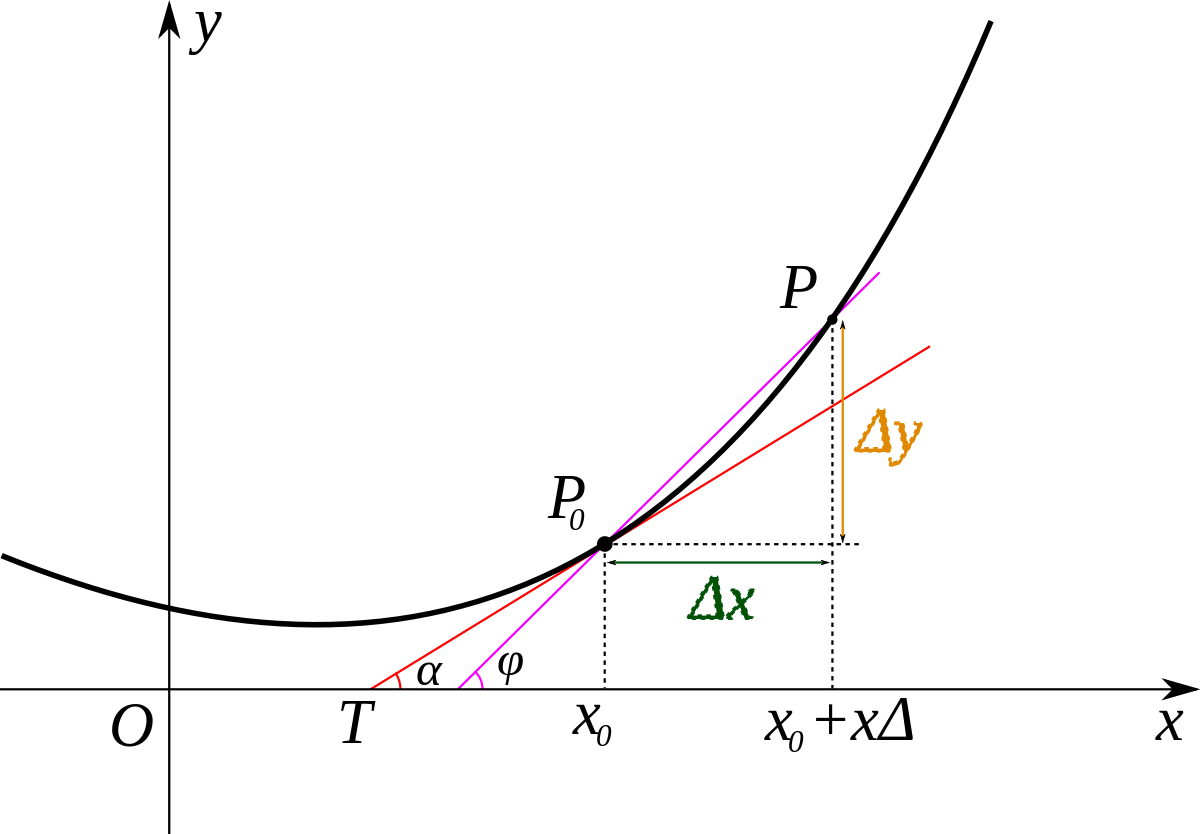
\includegraphics[width=6cm]{geoddx.png}
\end{figure}
\subsection*{{\fontfamily{qag}\selectfont 5. Conclusión}} \justify
Se  muestran de manera breve todas las expresiones anteriores para condensar lo visto en la fórmula esperada como una muestra de haber logrado algo muy tedioso de una manera muy intuitiva.
\end{document}